\documentclass{article}
\usepackage{times}
\usepackage[utf8]{inputenc}
\usepackage{graphicx}

\begin{document}
	
	
	\title{ORSI 1. beadandó feladat - dokumentáció} 
	\author{Kovács Bálint - FANW4Z}  %\texttt formats the text to a typewriter style font
	\date{\today}  %\today is replaced with the current date
	\maketitle
	
	\section{Feladat}
	A bemenet \texttt{input.txt} első sorában egy N pozitív egész olvasható, ennyi diáknak kell biztosítani termet, míg a következő N sorban a hallgatók NEPTUN-kódjai, azaz N string követi egymást, ez mutatja a jelentkezési sorrendet.
	
	Egy lehetséges bemeneti fájl:
	\begin{verbatim}
	7
	OSAVH1
	T0NDJB
	4S1UPL
	AXKAW4
	22TQP7
	NM8VPS
	PJVNEU
	\end{verbatim}
	
	A megoldás során TILOS a beépített rendezéseket használni (pl. \(std::sort()\)), a feladat egy párhuzamosított MergeSort (összefésüléses rendezés) implementálása! A fő folyamat feladata az adatok beolvasása az \texttt{input.txt} fájlból, majd az output.txt kimeneti fájl létrehozása, benne a rendezett adathalmazzal. Rendezéshez kötődő számítást ne végezzen! (Összefésülést sem!)

	
	\section{Felhasználói dokumentáció}
	
	\subsection{Környezet}
	A program futtatásához Erlang shell szükséges. 
	
	\subsection{Használat}
	Fordítsuk \(c(merge\_sort2)\) paranccsal, majd futtathatjuk \(merge\_sort2:start()\) függvényhívással. A fájl mellett kell elhelyezni az \texttt{input.txt} fájlt, melyet feldolgoz és az eredményt az \texttt{output.txt} nevű fájlba írja, a betűrend  alapján. Egy lehetséges bemenetet tartalmaz a mellékelt \texttt{input.txt} tesztfájl. Saját bemeneti fájlok esetén a sorok és a játékok számának pontos megadása nem fontos, elég ha az elején kihagyunk egy sort. Viszont  a helyes működéshez szükséges a többi sor megfelelő formátuma, és hogy ne legyen több üres sor a dokumentumban.
	
	\section{Fejlesztői dokumentáció}
	
	\subsection{A megoldás módja}
	A főfolyamat beolvassa az input fájlt, majd az olvasott adatra elindítja a párhuzamosított összefésülő rendezést. Ez később buborékrendezésre vált. A rendezett listát kiírjuk a folyamat végén. 
	
	\subsection{Implementáció}
	 A bemeneti adatokkal meghívjuk a \(merge\_sort\) függvényt, ami a rekurzív rendezésért felel. A beépített \(spawn()\) függvény segítségével a rendezés egyik ágát párhuzamosítjuk. Az összefésülő rendezés algoritmusa, mely alapján az említett függvényt írtam (dr. Fekete István oldaláról):\hfill \break
	 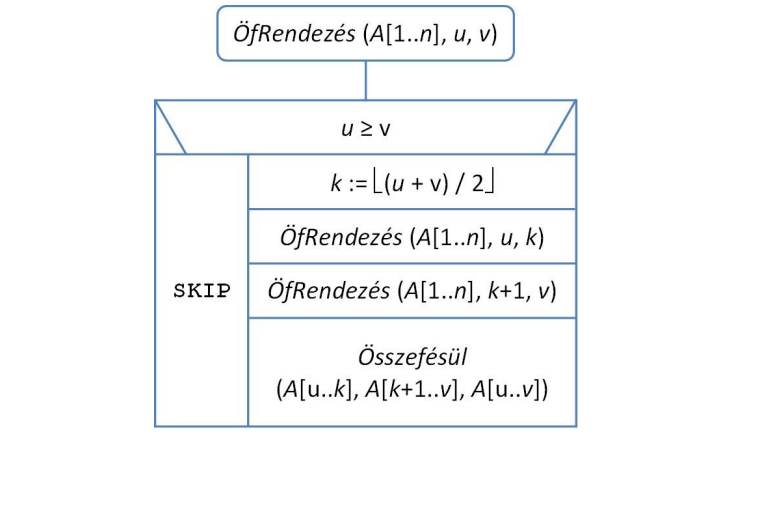
\includegraphics[scale=0.6]{mergeSort}
	 A futás egy makróban megadott értéknél (\(MergeLimit\)) rövidebb listákra buborékrendezésre vált. Ennek az értéknek a meghatározásról a tesztelés fázisban írok. A teljes implementáció egyetlen forrásfájlba szervezve, a \texttt{merge\_sort2.erl} fájlban található.
	
	\subsection{Fordítás}
	Fordítsunk \(c(merge\_sort2)\) paranccsal, majd futtathatjuk a programot \(merge\_sort2:start()\) függvényhívással.
	
	\subsection{Tesztelés}
	A programot 100000 sor hosszú fájllal teszteltem, ez volt az a méret, ahol látszódtak az eltérések a futási időben. Az eredmények, a buborék rendezésre váltást jelző szám függvényében, három futást átlagolva:
	\begin{itemize}
		\item 0 $\,\to\,$ 3,296s
		\item 5 $\,\to\,$  2,867s
		\item 20 $\,\to\,$  2,770s
		\item 40 $\,\to\,$   2,737s
		\item 70 $\,\to\,$   2,650s
		\item 100 $\,\to\,$   2,794s
	\end{itemize}
	Így 70re állítottam az értéket. Az érték különböző rendszereken eltérő lehet.
	
\end{document}